\subsubsection{Procedure}
Each participant was tested individually (see Figure \ref{fig:tt}). Besides the participant, a facilitator and an observer were also present. The test was split into seven parts.
\begin{figure*}[hbtp]
\centering
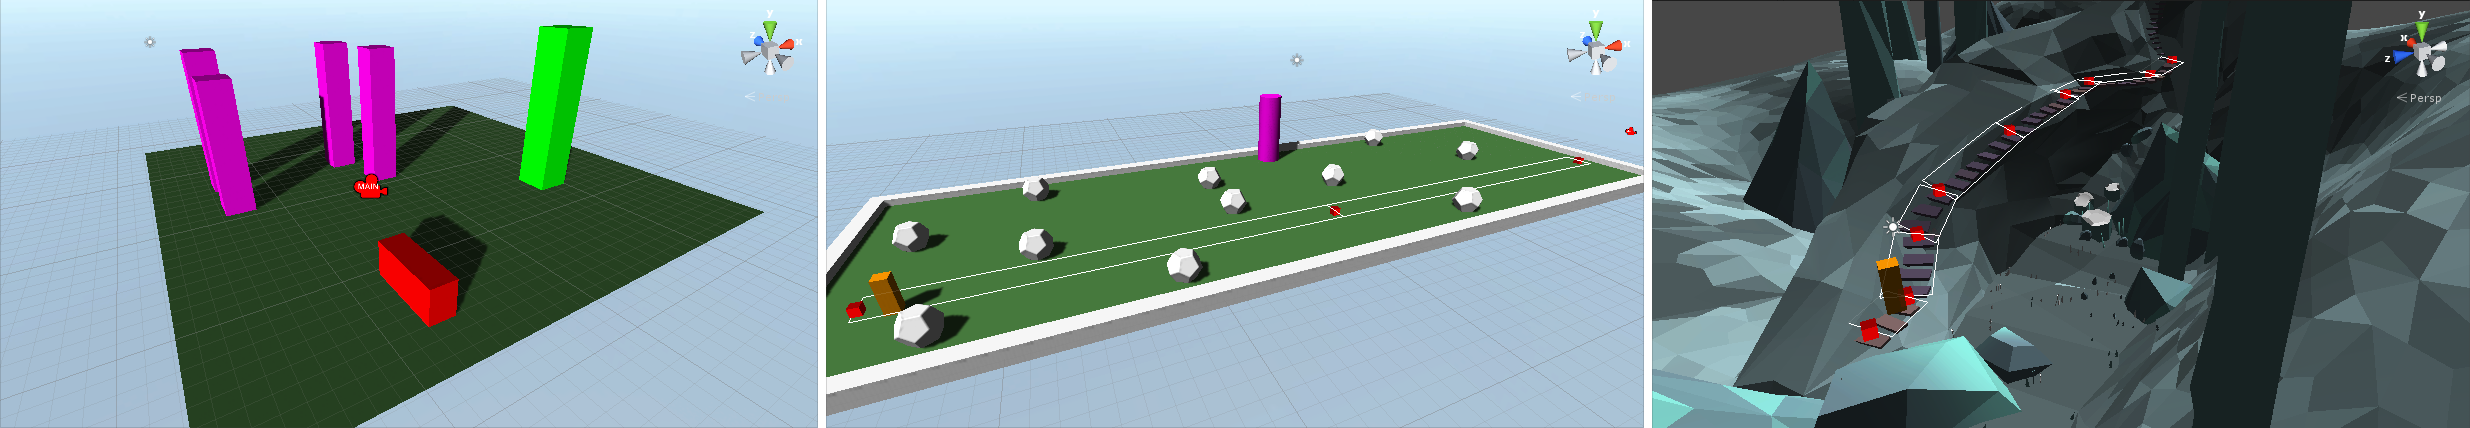
\includegraphics[width=0.8\textwidth]{Pics/sceneAll_horizontal}
\caption{The evaluation consisted of three parts, each with their own scene. The first scene was for getting a feel of basic navigation in Unity. The second scene was used for the test participants to try out the camera tool. The third scene was for the creative task where the test participants created their own framings.}
\label{fig:sceneAll}
\end{figure*}

\begin{enumerate}[noitemsep,nolistsep]
\item Introduction, Consent and Demographic
\item Trying the Camera Path Animator
\item Basic Navigation in Unity
\item Training with the FCT
\item Tasks with the FCT
\item Creative use of the FCT
\item Post-test Questionnaire
\end{enumerate}

The procedure was the same for all participants. The evaluation sessions lasted for approximately 50-60 minutes each.


\textbf{Introduction, Consent and Demographic}\\
The participants were given a brief introduction and presented a consent form to allow video recording. The participants started by answering a demographic questionnaire. 

\begin{figure}[htbp]
\centering
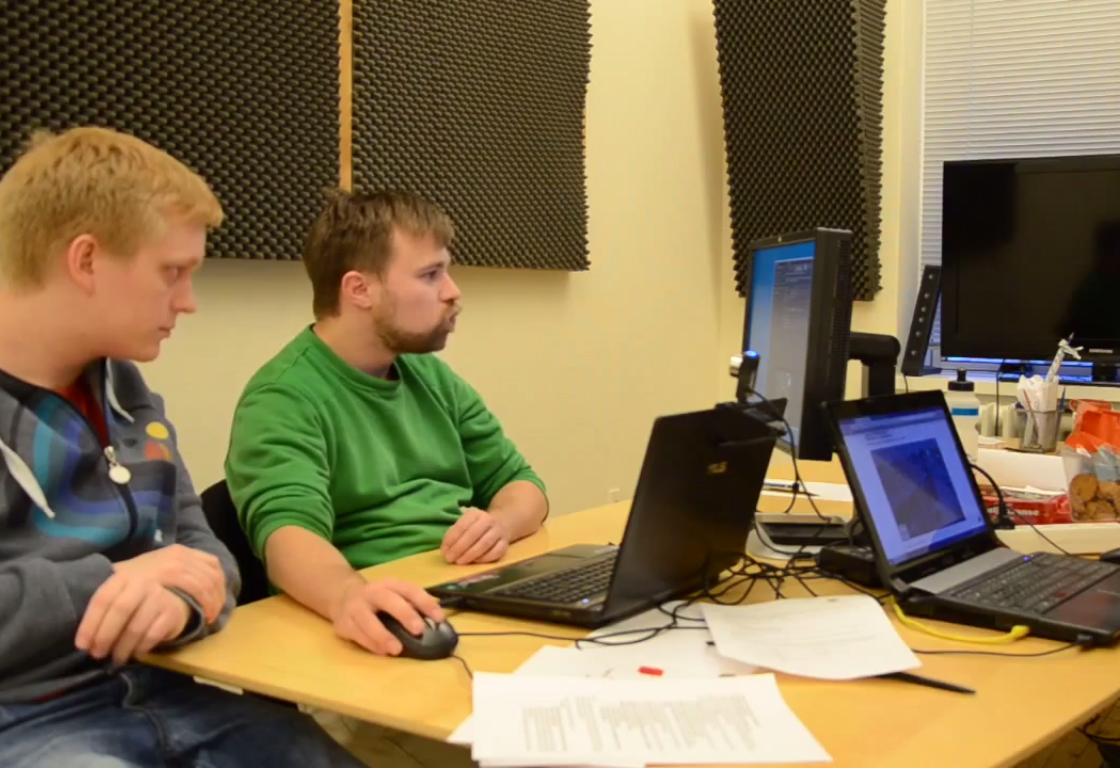
\includegraphics[width=0.3\textwidth]{Pics/test_setup}
\caption{The test participants used two monitors while working with FCT.}
\label{fig:tt}
\end{figure}

\textbf{Trying the Camera Path Animator}\\
The test participants were introduced to a small demo of the Camera Path Animator \cite{unity_camTool} (see Section \ref{relatedWork}). They were told to move the player character around and notice how the camera behaved accordingly. This was to give the participants a context for the evaluation test of the FCT, as well as introduce them to the concept of camera movements in an interactive environment.

%%



\textbf{Basic Navigation in Unity}\\
To ensure that all participants had a basic understanding of how to navigate in Unity, the facilitator gave a brief oral introduction to the basic functionality of Unity. This included a short description of the essential windows in Unity (scene view, game view, hierarchy and the inspector), as well as how to move and rotate objects. The participants were also instructed on how to move the scene view camera around in Unity. They were also told about Unity's \textit{Flythrough Mode} \cite{unity_flyMode}. To ensure that they actually understood how to navigate around, they were asked to move the camera to three specific locations in the scene. 

%For instance, they were told to place the camera on top of the green cube seen in Figure \ref{fig:sceneAll}.

This phase lasted around 2-5 minutes.

\textbf{Training with the FCT}\\
Before trying the FCT, the facilitator gave a short oral introduction of the framing concept by referring to a printout of Figure \ref{fig:framingConceptNew}. Afterwards, the participants were asked to open the FCT in Unity. Here, the facilitator went through all of the major features in a semi-structured way, explaining each feature one at a time, and having the test participants try each one.

A path was already defined in the scene. The test participants learned about how to place and adjust a framing. They learned how to create and move influence points. They then went through features such as changing the position and rotation of a camera using the different methods, i.e. changing the values by hand; using the \textit{be the camera} feature; using the \textit{snapshot} feature; and using the \textit{aim point}. In order to preview their changes, the participants were shown the \textit{interactive preview} and \textit{slider preview}. Afterwards, they were introduced to the graph editor, as well as miscellaneous smaller features.

This phase lasted around 15-20 minutes.

\textbf{Tasks with the FCT}\\
After the participants had tried out all of the major features in the FCT, they were handed a piece of paper with five tasks. These tasks required that the participants understood the concept about framings and knew how to create them using the tool. For each task, they were asked to create new framings.

\begin{enumerate}[noitemsep,nolistsep]
\item Make the camera's field of view change.
\item Make the camera tilt upwards.
\item Make the camera look at the tall pink cylinder.
\item Make the camera go from a low perspective to a bird's-eye view.
\item Change the interpolation of one of the previous assignments by changing the animation curve.
\end{enumerate} 

The chosen tasks reflect five common features and tasks that are often used when setting up a framing and a camera interpolation. The participants had to solve the tasks themselves; the facilitator only intervened when the participant was struggling with something, asked a question, or unforeseen errors occurred with the tool.

This phase lasted around 15-20 minutes.

\textbf{Creative use of the FCT}\\
After this, the participants were introduced to a level with a modelled environment. They were then tasked to envision and sketch two ways for the camera to move as the player character moved through this environment. After drawing their two sketches, they were tasked to implement both of these using our camera tool. The facilitator remained as neutral as possible for this part of the test, but still intervened if the participant was struggling or encountered things like bugs.


This phase lasted around 5-10 minutes.

\textbf{Post-test Questionnaire}\\
Finally, the test participants answered a short questionnaire about their experience with the FCT.

\begin{figure*}[htbp]
\centering
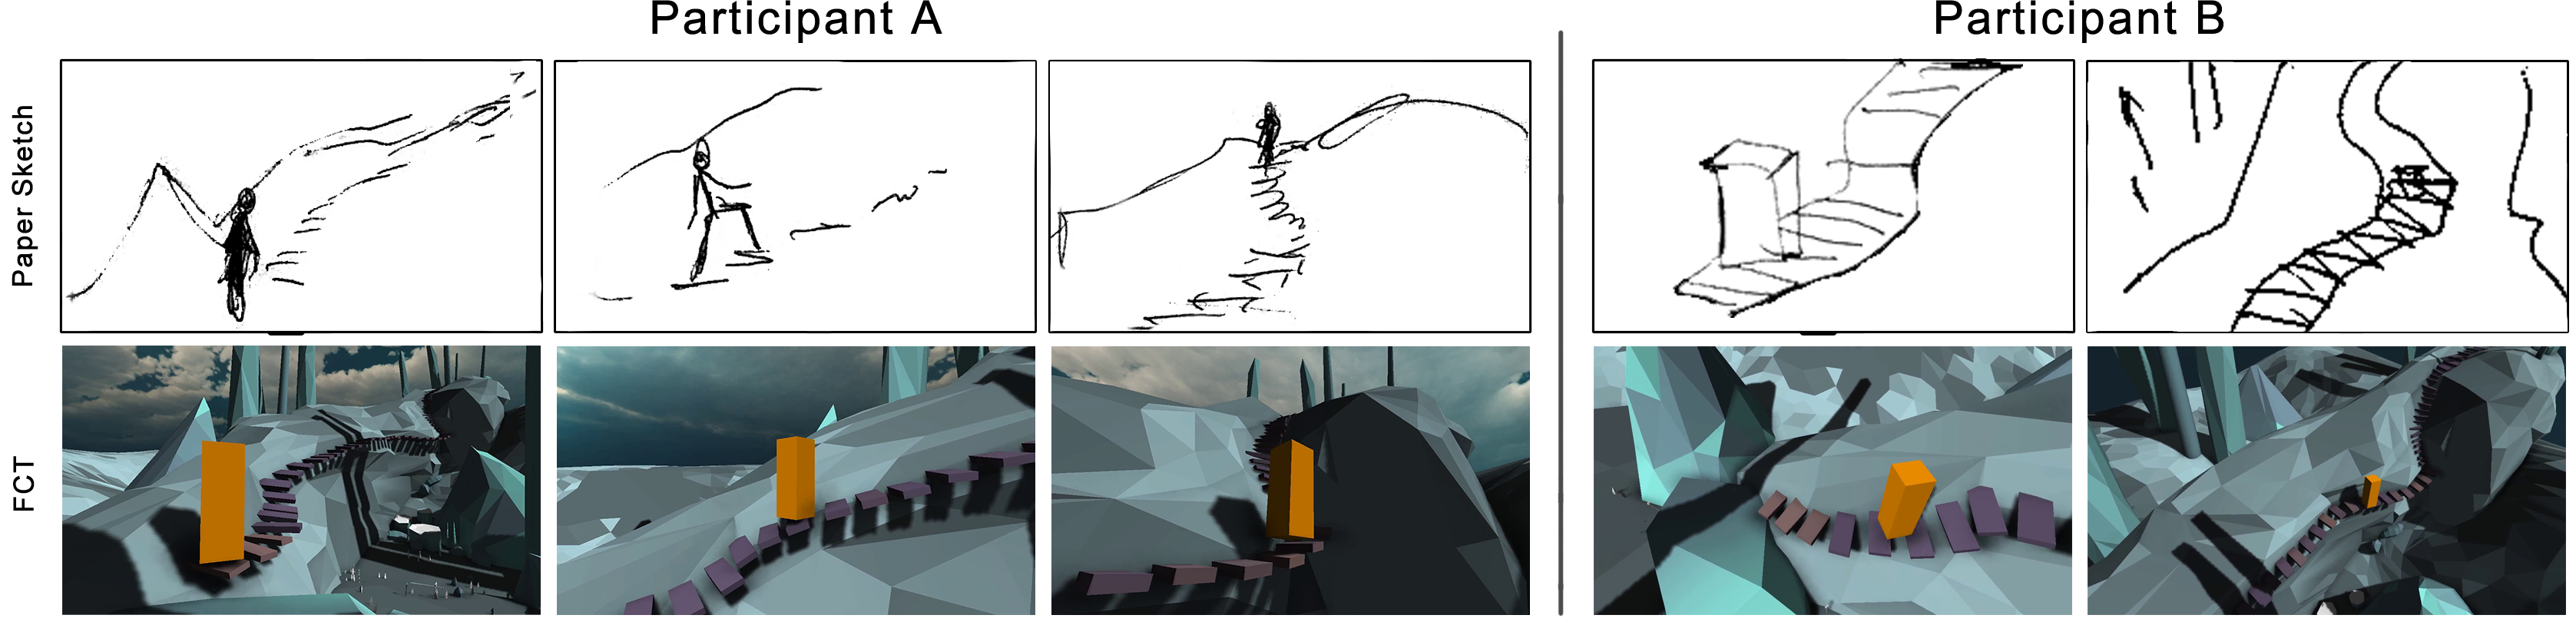
\includegraphics[width=0.9\textwidth]{Pics/Sketching_FramingsNew}
\caption{The participants drew sketches of camera movements in the creative phase during the evaluation. There were no restrictions of how to do this; but most drew traditional storyboards. This figure shows two different participants' sketches and implementations in FCT. Participant A had 4-6 years of Unity experience, while participant B had less then six months Unity experience.}
\label{fig:Sketching_Framings}
\end{figure*}